
% * Week 1. (Jul 27) Introduction and R boot camp (Rob & Souhaib)
%   - Lecture 1:  What is Business Analytics? Show case of R.
%   - Lab 1: R exercises
%   - Lecture 2: Introduction to R programming
% - R, Rstudio
% - Rmarkdown
% - Examples:
%     prediction: bulldozers
%     classification: see JWHAT
%     clustering
%   Business analytics vs data science vs statistics vs econometrics 
%   Venn diagrams



\documentclass[14pt]{beamer}
\usepackage{pgf,tikz,pgfpages,amsmath,bm,fancyvrb,animate}
\usepackage{graphicx,bera,booktabs,multicol}
\usepackage[australian]{babel}
\usepackage[utf8]{inputenc}
\usepackage{media9}
\usetikzlibrary{arrows}
\definecolor{mygreen}{rgb}{0,0.6,0}

\usepackage{verbatim}

\definecolor{Orange}{RGB}{255,140,0}
\long\def\TCorange#1{\textcolor{Orange}{#1}}
\long\def\TCblue#1{\textcolor{blue}{#1}}

\newcommand\Wider[2][3em]{%
\makebox[\linewidth][c]{%
  \begin{minipage}{\dimexpr\textwidth+#1\relax}
  \raggedright#2
  \end{minipage}%
  }%
}

\usetheme{Monash}
\def\ben{\begin{enumerate}[<+-| alert@+>]}
\def\een{\end{enumerate}}

%\AtBeginSubsection[]  
%  {  
%    \begin{frame}<*>{Outline}  
%      \tableofcontents[currentsection,currentsubsection]  
%    \end{frame}  
%  }


\graphicspath{{../figures/}{../figures/book_figures/Chapter2/}}

\title[Statistical learning]{Business Analytics}
\author{Week 2.\\ Assessing model accuracy}
\date{3 August 2015}

\DefineShortVerb{\"}
\def\FancyVerbFormatCom{\color[rgb]{0.6,0,1}\relax}


\def\source#1{\vspace{-0.4cm}\par{\fontsize{6}{8}\sffamily \url{#1}}}
\def\inlinesource#1{\hbox{\fontsize{6}{8}\sffamily \url{#1}}}

 
\begin{document}

\begin{frame}[plain]{}
\maketitle
\begin{textblock}{11}(0.5,1.3){\color{white}\large
\textbf{ETC3250}}
\end{textblock}


\end{frame}

\section{Regression problems}

\begin{frame}{Assessing model accuracy}
Suppose we have a regression model $y=f(x)+\varepsilon$. Estimate
$\hat{f}$ from some \textbf{training} data, $Tr=\{x_i,y_i\}_1^n$.

One common measure of accuracy is:
\begin{block}{Training Mean Squared Error}
\[
\text{MSE}_{Tr} = \mathop{\text{Ave}}\limits_{i\in Tr}[y_i-\hat{f}(x_i)]^2 =
\frac{1}{n}\sum_{i=1}^n [(y_i-\hat{f}(x_i)]^2
\]
\end{block}
\pause

%\only<2->{\begin{alertblock}{Problem:}
%A small MSE on the training data does not guarantee a small MSE on the test data.
%\end{alertblock}}

\only<2->{Better to compute it using \textbf{test} data $Te=\{x_j,y_j\}_1^m$
\begin{block}{Test Mean Squared Error}
\[
\text{MSE}_{Te} = \mathop{\text{Ave}}\limits_{j\in Te}[y_j-\hat{f}(x_j)]^2 =
\frac{1}{m}\sum_{j=1}^m [(y_j-\hat{f}(x_j)]^2
\]
\end{block}
}

\vspace*{10cm}

\end{frame}
\begin{frame}{Training vs Test MSEs}
\begin{itemize}
\item In general, the more \emph{flexible} a method is, the lower its
\emph{training MSE} will be. i.e. it will “fit” the training data very well.

\item However, the test MSE may be higher for a more flexible method than for a simple approach like linear regression. 

\item Flexibility also makes interpretation more difficult. There is
a trade-off between flexibility and model interpretability.
\end{itemize}
\end{frame}

\begin{frame}{Example: splines}
\placefig{0.2}{1}{width=12.2cm}{2-9-crop.pdf}
\begin{textblock}{6}(0.2,7.8)\small
Black: true curve\\
Orange: linear regression\\
Blue/green: Smoothing splines
\end{textblock}
\begin{textblock}{6.5}(7.2,7.8)\small
Grey: Training MSE\\
Red: Test MSE\\
Dashed: Minimum test MSE
\end{textblock}
\end{frame}

\begin{frame}{Example: splines}
\placefig{0.2}{1}{width=12.2cm}{2-10-crop.pdf}
\begin{textblock}{6}(0.2,7.8)\small
Black: true curve\\
Orange: linear regression\\
Blue/green: Smoothing splines
\end{textblock}
\begin{textblock}{6.5}(7.2,7.8)\small
Grey: Training MSE\\
Red: Test MSE\\
Dashed: Minimum test MSE
\end{textblock}
\end{frame}


\begin{frame}{Example: splines}
\placefig{0.2}{1}{width=12.2cm}{2-11-crop.pdf}
\begin{textblock}{6}(0.2,7.8)\small
Black: true curve\\
Orange: linear regression\\
Blue/green: Smoothing splines
\end{textblock}
\begin{textblock}{6.5}(7.2,7.8)\small
Grey: Training MSE\\
Red: Test MSE\\
Dashed: Minimum test MSE
\end{textblock}
\end{frame}


\begin{frame}{Bias-variance tradeoff}
\begin{alertblock}{}
There are two competing forces that govern the
choice of learning method: \textbf{bias} and \textbf{variance}. 
\end{alertblock}

\begin{block}{Bias}
is the error that is introduced by modeling a 
complicated problem by a simpler problem.
\end{block}
\begin{itemize}
\item For example, linear regression assumes a linear relationship when few real relationships are exactly linear.
\item In general, the more flexible a method is, the less bias it will have. 
\end{itemize}
\vspace*{10cm}

\end{frame}

\begin{frame}{Bias-variance tradeoff}
\begin{alertblock}{}
There are two competing forces that govern the
choice of learning method: \textbf{bias} and \textbf{variance}. 
\end{alertblock}

\begin{block}{Variance}
refers to how much your estimate would change if you had different training data.
\end{block}
\begin{itemize}
\item In general, the more flexible a method is, the more variance it has. 
\end{itemize}

\vspace*{10cm}
\end{frame}

\begin{frame}{The bias-variance tradeoff}

\begin{alertblock}{MSE decomposition}
If $Y = f(x) + \varepsilon$ and $f(x)=\text{E}[Y\mid X=x]$, then the expected \textbf{test} MSE for a new $Y$ at $x_0$ will be equal to\vspace*{-0.3cm}
$$\text{E}[(Y-\hat{f}(x_0))^2] = [\text{Bias}(\hat{f}(x_0))]^2 + \text{Var}(\hat{f}(x_0)) + \text{Var}(\varepsilon)$$
\end{alertblock}
\begin{block}{}
Test MSE = Bias$^2$ + Variance + Irreducible variance
\end{block}
\begin{itemize}
\item The expectation averages over the variability of $Y$ as well as the variability in the training data.
\item As the flexibility of $\hat{f}$ increases, its variance increases and its bias decreases.
\item Choosing the flexibility based on average test MSE amounts to a \structure{bias-variance trade-off}.
\end{itemize}
\end{frame}

\begin{frame}{Bias-variance trade-off}
\placefig{0.9}{1}{width=3cm, trim=0 0 280 0, clip=true}{2-9-crop.pdf}
\placefig{4.2}{1}{width=3cm, trim=0 0 280 0, clip=true}{2-10-crop.pdf}
\placefig{8.4}{1}{width=3cm, trim=0 0 280 0, clip=true}{2-11-crop.pdf}
\placefig{1}{4.4}{width=10.4cm}{2-12-crop}
\end{frame}

\begin{frame}{Optimal prediction}
\begin{alertblock}{MSE decomposition}
If $Y = f(x) + \varepsilon$ and $f(x)=\text{E}[Y\mid X=x]$, then the expected \textbf{test} MSE for a new $Y$ at $x_0$ will be equal to\vspace*{-0.3cm}
$$\text{E}[(Y-\hat{f}(x_0))^2] = [\text{Bias}(\hat{f}(x_0))]^2 + \text{Var}(\hat{f}(x_0)) + \text{Var}(\varepsilon)$$
\end{alertblock}

The optimal MSE is obtained when 
\begin{block}{}
\centerline{$\hat{f}=f = \text{E}[Y\mid X=x].$}
\end{block}
Then bias=variance=0 and
\begin{block}{}
\centerline{$\text{MSE} = \text{irreducible variance}$}
\end{block}
This is called the \alert{``oracle'' predictor} because it is not achievable in practice.

\end{frame}

\section{Classification problems}

\begin{frame}{Classification problems}

Here the response variable $Y$ is \alert{qualitative}.
\begin{itemize}
\item e.g., email is one of ${\cal C} = (\text{spam},\text{ham})$
\item e.g., voters are one of ${\cal C} = (\text{Liberal},\text{Labor},\text{Green},\text{National},\text{Other})$
\end{itemize}\pause
\structure{Our goals are:}
\begin{enumerate}
\item Build a classifier $C(x)$ that assigns a class label from ${\cal C}$ to a future unlabeled observation $x$.
\item Assess the uncertainty in each classification (i.e., the probability of misclassification).
\item Understand the roles of the different predictors among $X = (X_1,X_2,\dots,X_p)$.
\end{enumerate}
\end{frame}

\begin{frame}{Classification problem}

In place of MSE, we now use:
\begin{block}{Error rate}
$$
\text{Error rate} = \frac{1}{n}\sum_{i=1}^n I(y_i \ne \hat{f}(x_i))
$$
\end{block}
where $\hat{f}(x_i)$ is the predicted class label

and  $I(y_i\ne \hat{f}(x_i))$ is an indicator function.\pause
\begin{itemize}
\item That is, the error rate is the fraction of misclassifications.
\item The training error rate is misleading (too small).
\item We want to minimize the test error rate:
$
\text{E}(I(y_0 \ne \hat{y}_0))
$
\end{itemize}

\end{frame}

\begin{frame}{Optimal classifier}

Suppose the $K$ elements in $\cal C$ are
numbered $1, 2, \dots, K$. Let
\begin{block}{}
\centerline{$
p_k(x) = \text{Pr}(Y = k\mid X = x),\qquad k = 1, 2, \dots , K.
$}
\end{block}
These are the \alert{conditional class probabilities} at $x$. \pause


Then the \alert{Bayes} classifier at $x$ is
\begin{block}{}
\centerline{$
C(x) = j\quad \text{if $p_j(x) = \max\{p_1(x), p_2(x), \dots, p_K(x)\}$}
$}
\end{block}\pause

\begin{itemize}
\item 
This gives the minimum average test error rate. 
\item It is an ``oracle predictor'' because we do not usually know $p_k(x)$.
\end{itemize}
\end{frame}

\begin{frame}{Bayes error rate}
\begin{block}{Bayes error rate}
\centerline{$1-\text{E}\left(\max_j \text{Pr}(Y=j | X)\right)$}
\end{block}
\begin{itemize}
\item The ``Bayes error rate'' is the lowest possible error rate that could be achieved if we knew exactly the ``true'' probability distribution of the data.
\item It is analagous to the ``irreducible error'' in regression.
\item On test data, no classifier can get lower error rates than the Bayes error rate.
\item In reality, the Bayes error rate is not known exactly.
\end{itemize}
\end{frame}

\begin{frame}{Bayes optimal classifier}
\fullheight{2-13}
\end{frame}

\begin{frame}{k-Nearest Neighbours}

One of the simplest classifiers. Given a test observation $x_0$:
\begin{itemize}
\item Find the $K$ nearest points to $x_0$ in the training data: ${\cal N}_0$.
\item Estimate conditional probabilities
$$\text{Pr}(Y=j \mid X=x_0) = \frac{1}{K}\sum_{i\in {\cal N}_0} I(y_i = j).$$
\item Apply Bayes rule and classify $x_0$ to class with largest probability.
\end{itemize}
\end{frame}

\begin{frame}{kNN Classifier}
\fullwidth{2-14}
\begin{textblock}{10}(0.5,8.4)
$K=3$.
\end{textblock}
\end{frame}


\begin{frame}{kNN Classifier}
\fullheight{2-15}
\end{frame}

\begin{frame}{kNN Classifier}
\fullwidth{2-16}
\end{frame}


\begin{frame}{kNN Classifier}
\fullheight{2-17}
\end{frame}


\begin{frame}{A fundamental picture}
\fullwidth{bias-var-tradeoff.png}

\only<2->{\begin{textblock}{2}(5.5,6.1)

\begin{tikzpicture}
\node (0) at (0,0) {\textcolor{purple}{\textbf{Best trade}}};
\path[->,draw=purple,solid,line width=2pt,fill=purple] (0,0.4) -- (0,1.8);
\end{tikzpicture}
\end{textblock}}

\only<3>{\begin{textblock}{2}(2,5.5)
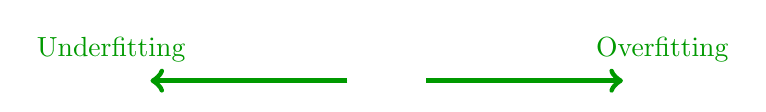
\begin{tikzpicture}
\node (0) at (-3.5,0.4) {\textcolor{mygreen}{Underfitting}};
\node (0) at (3.5,0.4) {\textcolor{mygreen}{Overfitting}};
\path[->,draw=mygreen,solid,line width=2pt,fill=mygreen] (-0.5,0) -- (-3,0);
\path[->,draw=mygreen,solid,line width=2pt,fill=mygreen] (0.5,0) -- (3,0);
\end{tikzpicture}
\end{textblock}}

\end{frame}



\end{document}


%\input{temp.tex}